\documentclass[a4paper,11pt]{article}
\usepackage{graphicx, amsfonts, amstext, amsmath, amssymb, amsthm, authblk}
\usepackage{amsthm}
\usepackage{verbatim,rotating,enumitem}
\usepackage{color,pst-text,amsmath, amssymb, amsthm, pst-node, verbatim, subfigure}
\usepackage{multicol}
\usepackage{textcomp}
\usepackage[stable]{footmisc}
\usepackage{lscape}

% \usepackage[framed,numbered,autolinebreaks,useliterate]{mcode}
% \newtheorem{algorithm}{Algorithm}
% ========================================
% Packages for flow chart. 
% \usepackage[latin1]{inputenc}
% \usepackage{tikz}
% \usetikzlibrary{shapes,arrows}
% \usepackage{verbatim}
% \usepackage[active,tightpage]{preview}
% \PreviewEnvironment{tikzpicture}
% \setlength\PreviewBorder{5pt}%
% =======================================
% \newcommand{\h}{\hspace{.8cm}}
%opening


\author{A.H. Sheikh}

% \email{hanangul12@yahoo.co.uk}
% \affiliation{Delft Institute of Applied Mathematics, Delft University of
% Technology, Netherlands}
 
% \institution{Delft University of Technology, Netherlands}
% \title{Meeting discussion}
\title{Instruction for ADEF1 Solver Software}
\vspace{20cm}
\date{}
% \date{\today}
\begin{document}
%
\maketitle
%
\section{Introduction}
ADEF1 solver software is divided into two parts. Multilvel implementation
requires matrices at all levels from finest to coarsest. The data files are
constructed in Matlab and subsequently are written into \texttt{.DAT} files.
Important part of ADEF1 solver sotware is part which implements multilevel
preconditioner. This is implemented in \texttt{PETSc}, which calls the 
\texttt{.DAT} files on run time. 
\subsection{Structure}
Main directory  \texttt{Adef1\_Software} contains two sub-directorows;
\texttt{ConstructDatFiles} and \texttt{PetscSolver}.\\
The directory \texttt{ConstructDatFiles} constructs data files. 
\section{Constructing DATA files}
AddPath of your PETSC"matlab-bin" directory in matlab session
or adapt path in program "MainMarmousi.m" . 


Run the program "MainMarmousi.m"
It will ask for options in an input dialogue box. 
Options: 

-- 	Frequency "f", give values f = 1, 10, 20 or 40

--	Meshsize, in terms of grid points per wavelenth. Limited to 10 or 20.

--	Real shift in complex shifted Laplace preconditioenrr CSLP. Choose
whatever you want to 
	use as CSLP. 

--	Real shift in complex shifted Laplace preconditioenrr CSLP. Choose
whatever you want to 
	use as CSLP. 

--	Imaginary shift in complex shifted Laplace preconditioenrr CSLP. Choose
whatever you want to 
	use as CSLP. 

--	Damping parameter in equation. 


First test run with defaults option in order to check if it runs smoothly. 
Subsequently customize with options. 

Output file will be a .DAT file and will be saved in directory ../DAtaFiles/ 
with customized name  "f1gpWL10a0.05" where 

-----------------------------------------------------------------------------
f			tells frequency
-----------------------------------------------------------------------------
1 (or 10,20,40)	 	provided frequency
-----------------------------------------------------------------------------
gpWL			indicates mesh size in terms gridpoints / wavelength
-----------------------------------------------------------------------------
10 (or 20)		provided grid points / wavelength
-----------------------------------------------------------------------------
a			damping parameter $\alpha$
-----------------------------------------------------------------------------
0.05			provided damping parameter value
-----------------------------------------------------------------------------




==========================
PLEASE NOTE WHEN ADAPTING
==========================
Reading .dat file in Petsc is sensible of orders of things(matrices and
vectors) 
written in .dat file . 

If you wish to adapt, adapt it carefully. Take care of the order, 
persist with same order while writing into .dat file and reading same .dat file.


Run the Matlab program \texttt{MainMarmousi.m} in matlab session. This will
immediately ask the options and will construct discrete matrices accordingly.
An example is shown in Figure \ref{fig:fig1}.
%
\begin{figure}[h]
\centering
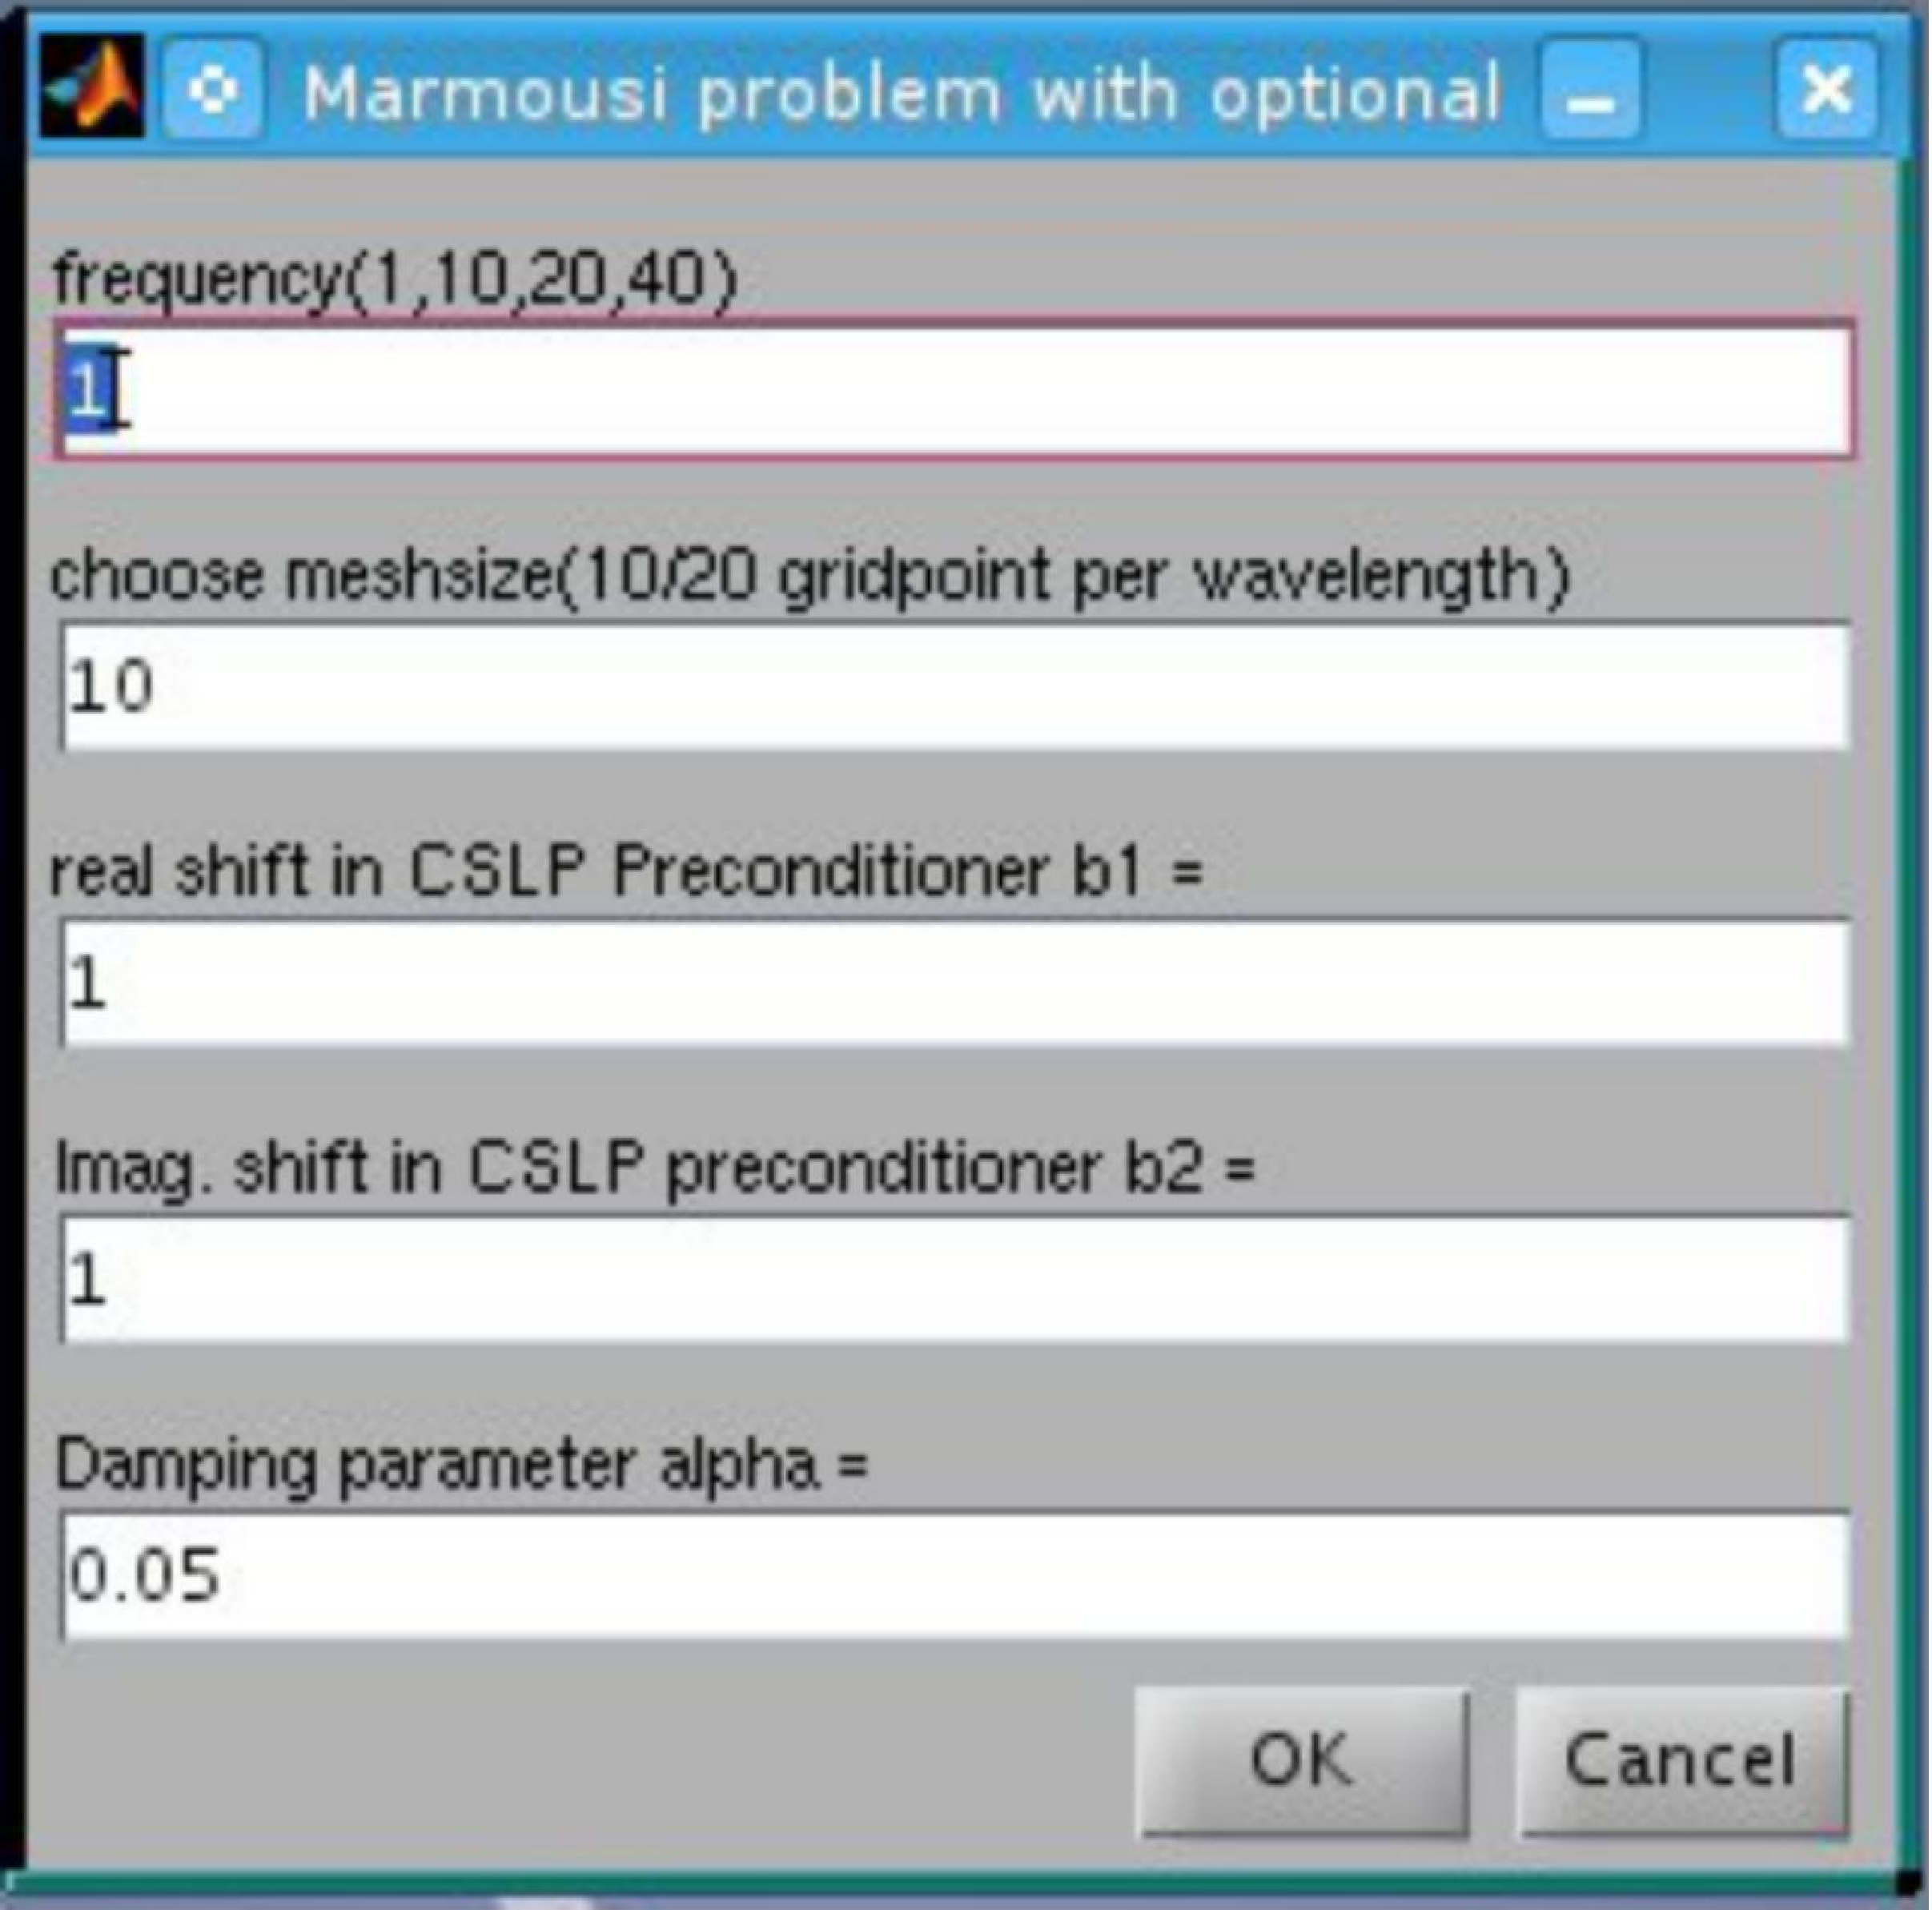
\includegraphics[width=7cm,height=5cm]{image1.pdf}
\caption{Menu to choose options while constructing \texttt{.DAT} files.}
\label{fig:fig1}
\end{figure}
\\



% \input{random.tex}
% %
% \input{petsc-email}
% %
% \input{20Sep.tex}
% % %
% \input{ToDo.tex}
% %
% \input{ToNote.tex}
% % %
% \input{algorithm-explore.tex}
% % %
% \input{petsc.tex}
% % 
%  % 
% %
% \cleardoublepage
% %
% % \input{petsc1.tex}
% %
% \input{3d7pntFDM.tex}
% 
% 
%  \newpage
%  \bibliography{reference}
%   \bibliographystyle{unsrt}
%    \bibliographystyle{abbrv}
%     \newpage
% %	

%
\end{document}
